
% Programming/Coding Assignment
% LaTeX Template
%
% This template has been downloaded from:
% http://www.latextemplates.com
%
% Original author:
% Ted Pavlic (http://www.tedpavlic.com)
%
% Note:
% The \lipsum[#] commands throughout this template generate dummy text
% to fill the template out. These commands should all be removed when 
% writing assignment content.
%
% This template uses a Perl script as an example snippet of code, most other
% languages are also usable. Configure them in the "CODE INCLUSION 
% CONFIGURATION" section.
%
%%%%%%%%%%%%%%%%%%%%%%%%%%%%%%%%%%%%%%%%%

%----------------------------------------------------------------------------------------
%   PACKAGES AND OTHER DOCUMENT CONFIGURATIONS
%----------------------------------------------------------------------------------------

\documentclass{article}

\usepackage{fancyhdr} % Required for custom headers
\usepackage{lastpage} % Required to determine the last page for the footer
\usepackage{extramarks} % Required for headers and footers
\usepackage[usenames,dvipsnames]{color} % Required for custom colors
\usepackage{graphicx} % Required to insert images
\usepackage{listings} % Required for insertion of code
\usepackage{courier} % Required for the courier font
\usepackage{lipsum} % Used for inserting dummy 'Lorem ipsum' text into the template
\usepackage{fullpage,amsthm,amsfonts,amssymb,epsfig,amsmath}

% Margins
\topmargin=-0.45in
\evensidemargin=0in
\oddsidemargin=0in
\textwidth=6.5in
\textheight=9.0in
\headsep=0.25in

\linespread{1.1} % Line spacing

% Set up the header and footer
\pagestyle{fancy}
\lhead{\hmwkAuthorName} % Top left header
\chead{\hmwkClass\ (\hmwkClassInstructor\ \hmwkClassTime): \hmwkTitle} % Top center head
\rhead{\firstxmark} % Top right header
\lfoot{\lastxmark} % Bottom left footer
\cfoot{} % Bottom center footer
\rfoot{Page\ \thepage\ of\ \protect\pageref{LastPage}} % Bottom right footer
\renewcommand\headrulewidth{0.4pt} % Size of the header rule
\renewcommand\footrulewidth{0.4pt} % Size of the footer rule
\newcommand{\tab}{\hspace*{3em}}

\setlength\parindent{0pt} % Removes all indentation from paragraphs

%----------------------------------------------------------------------------------------
%   CODE INCLUSION CONFIGURATION
%----------------------------------------------------------------------------------------

\definecolor{MyDarkGreen}{rgb}{0.0,0.4,0.0} % This is the color used for comments
\lstloadlanguages{Perl} % Load Perl syntax for listings, for a list of other languages supported see: ftp://ftp.tex.ac.uk/tex-archive/macros/latex/contrib/listings/listings.pdf
\lstset{language=Perl, % Use Perl in this example
        frame=single, % Single frame around code
        basicstyle=\small\ttfamily, % Use small true type font
        keywordstyle=[1]\color{Blue}\bf, % Perl functions bold and blue
        keywordstyle=[2]\color{Purple}, % Perl function arguments purple
        keywordstyle=[3]\color{Blue}\underbar, % Custom functions underlined and blue
        identifierstyle=, % Nothing special about identifiers                                         
        commentstyle=\usefont{T1}{pcr}{m}{sl}\color{MyDarkGreen}\small, % Comments small dark green courier font
        stringstyle=\color{Purple}, % Strings are purple
        showstringspaces=false, % Don't put marks in string spaces
        tabsize=5, % 5 spaces per tab
        %
        % Put standard Perl functions not included in the default language here
        morekeywords={rand},
        %
        % Put Perl function parameters here
        morekeywords=[2]{on, off, interp},
        %
        % Put user defined functions here
        morekeywords=[3]{test},
        %
        morecomment=[l][\color{Blue}]{...}, % Line continuation (...) like blue comment
        numbers=left, % Line numbers on left
        firstnumber=1, % Line numbers start with line 1
        numberstyle=\tiny\color{Blue}, % Line numbers are blue and small
        stepnumber=5 % Line numbers go in steps of 5
}

% Creates a new command to include a perl script, the first parameter is the filename of the script (without .pl), the second parameter is the caption
\newcommand{\perlscript}[2]{
\begin{itemize}
\item[]\lstinputlisting[caption=#2,label=#1]{#1.pl}
\end{itemize}
}

%----------------------------------------------------------------------------------------
%   DOCUMENT STRUCTURE COMMANDS
%   Skip this unless you know what you're doing
%----------------------------------------------------------------------------------------

% Header and footer for when a page split occurs within a problem environment
\newcommand{\enterProblemHeader}[1]{
\nobreak\extramarks{#1}{#1 continued on next page\ldots}\nobreak
\nobreak\extramarks{#1 (continued)}{#1 continued on next page\ldots}\nobreak
}

% Header and footer for when a page split occurs between problem environments
\newcommand{\exitProblemHeader}[1]{
\nobreak\extramarks{#1 (continued)}{#1 continued on next page\ldots}\nobreak
\nobreak\extramarks{#1}{}\nobreak
}

\setcounter{secnumdepth}{0} % Removes default section numbers
\newcounter{homeworkProblemCounter} % Creates a counter to keep track of the number of problems

\newcommand{\homeworkProblemName}{}
\newenvironment{homeworkProblem}[1][Problem \arabic{homeworkProblemCounter}]{ % Makes a new environment called homeworkProblem which takes 1 argument (custom name) but the default is "Problem #"
\stepcounter{homeworkProblemCounter} % Increase counter for number of problems
\renewcommand{\homeworkProblemName}{#1} % Assign \homeworkProblemName the name of the problem
\section{\homeworkProblemName} % Make a section in the document with the custom problem count
\enterProblemHeader{\homeworkProblemName} % Header and footer within the environment
}{
\exitProblemHeader{\homeworkProblemName} % Header and footer after the environment
}

\newcommand{\problemAnswer}[1]{ % Defines the problem answer command with the content as the only argument
\noindent\framebox[\columnwidth][c]{\begin{minipage}{0.98\columnwidth}#1\end{minipage}} % Makes the box around the problem answer and puts the content inside
}

\newcommand{\homeworkSectionName}{}
\newenvironment{homeworkSection}[1]{ % New environment for sections within homework problems, takes 1 argument - the name of the section
\renewcommand{\homeworkSectionName}{#1} % Assign \homeworkSectionName to the name of the section from the environment argument
\subsection{\homeworkSectionName} % Make a subsection with the custom name of the subsection
\enterProblemHeader{\homeworkProblemName} % Header and footer within the environment
}{
\enterProblemHeader{\homeworkProblemName} % Header and footer after the environment
}

%----------------------------------------------------------------------------------------
%   NAME AND CLASS SECTION
%----------------------------------------------------------------------------------------

\newcommand{\hmwkTitle}{Homework\ \#4} % Assignment title
\newcommand{\hmwkDueDate}{Tuesday,\ April\ 28st,\ 2015} % Due date
\newcommand{\hmwkClass}{CMPS\ 102} % Course/class
\newcommand{\hmwkClassTime}{4:00pm} % Class/lecture time
\newcommand{\hmwkClassInstructor}{Warmuth} % Teacher/lecturer
\newcommand{\hmwkAuthorName}{John Allard \ 1437547} % Your name


%----------------------------------------------------------------------------------------
%----------------------------------------------------------------------------------------
%   USER SETTINGS
%----------------------------------------------------------------------------------------
%----------------------------------------------------------------------------------------
\usepackage{mathtools}
\DeclarePairedDelimiter\ceil{\lceil}{\rceil}
\DeclarePairedDelimiter\floor{\lfloor}{\rfloor}



%----------------------------------------------------------------------------------------
%   TITLE PAGE
%----------------------------------------------------------------------------------------

\title{
\vspace{2in}
\textmd{\textbf{\hmwkClass:\ \hmwkTitle}}\\
\normalsize\vspace{0.1in}\small{Due\ on\ \hmwkDueDate}\\
\vspace{0.1in}\large{\textit{}}
\vspace{3in}
}

\author{\textbf{\hmwkAuthorName}}
\date{} % Insert date here if you want it to appear below your name

%----------------------------------------------------------------------------------------

\begin{document}

\maketitle

%----------------------------------------------------------------------------------------
%   TABLE OF CONTENTS
%----------------------------------------------------------------------------------------

%\setcounter{tocdepth}{1} % Uncomment this line if you don't want subsections listed in the ToC

% \tableofcontents
\newpage





%----------------------------------------------------------------------------------------
%   PROBLEM 1
%----------------------------------------------------------------------------------------

% To have just one problem per page, simply put a \clearpage after each problem

\begin{homeworkProblem}

Suppose Dijkstra's algorithm is run on the following graph, starting at node A. \\

\begin{center}
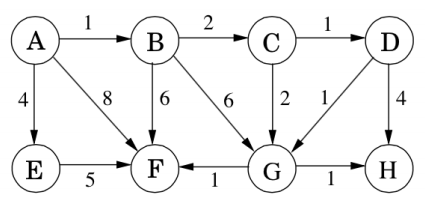
\includegraphics[width=3in]{DPV41.PNG}
\end{center}

\begin{enumerate}

\item Draw a table showing the intermediate distance values of all the nodes at each iteration of the algorithm. \\    

% \begin{tabular}{|c|c|c|c|c|c|c|c|c|} \hline
%        &   a   &   b   &   c   &   d   &   e   &   f   &   g   &   h   \\ \hline
%    a   &   0   &   6   &   .   &   .   &   1   &   .   &   .   &   .   \\ \hline
%    b   &   6   &   0   &   5   &   .   &   2   &   2   &   .   &   .   \\ \hline
%    c   &   .   &   5   &   0   &   6   &   .   &   5   &   4   &   .   \\ \hline
%    d   &   .   &   .   &   6   &   0   &   .   &   .   &   5   &   7   \\ \hline
%    e   &   1   &   2   &   .   &   .   &   0   &   1   &   .   &   .   \\ \hline
%    f   &   .   &   2   &   5   &   .   &   1   &   0   &   3   &   .   \\ \hline
%    g   &   .   &   .   &   4   &   5   &   .   &   3   &   0   &   3   \\ \hline
%    h   &   .   &   .   &   .   &   7   &   .   &   .   &   3   &   3   \\ \hline
% \end{tabular} 

The table below shows each iteration as a row, with later iterations being below earlier iterations. The numbers in each table section represent the shortest distance knows from the source (vertex A) to the vertex corresponding to that column during the iteration given by the row number. The distances to A are always zero because A is the source. For brevity, I use a `.' instead of an $\infty$ to represent infinite distances.

\begin{tabular}{|c|c|c|c|c|c|c|c|c|} \hline
 d(x) &   a   &   b   &   c   &   d   &   e   &   f   &   g   &   h   \\ \hline
      &   0   &   .   &   .   &   .   &   .   &   .   &   .   &   .   \\ \hline
      &   0   &   1   &   .   &   .   &   4   &   8   &   .   &   .   \\ \hline
      &   0   &   1   &   3   &   .   &   4   &   7   &   7   &   .   \\ \hline
      &   0   &   1   &   3   &   4   &   4   &   7   &   5   &   4   \\ \hline
      &   0   &   1   &   3   &   4   &   4   &   7   &   5   &   4   \\ \hline
      &   0   &   1   &   3   &   4   &   4   &   7   &   5   &   4   \\ \hline
      &   0   &   1   &   3   &   4   &   4   &   6   &   5   &   4   \\ \hline
      &   0   &   1   &   3   &   4   &   4   &   6   &   5   &   4   \\ \hline
\end{tabular} 


\item Show the final shortest-path tree. \\

\begin{center}
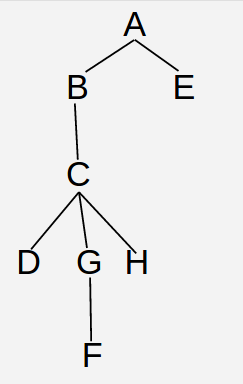
\includegraphics[width=2in]{sssp_tree.png}
\end{center}


\end{enumerate}


\end{homeworkProblem}






%----------------------------------------------------------------------------------------
%   PROBLEM 2
%----------------------------------------------------------------------------------------

\begin{homeworkProblem}

Consider the following graph \\

\begin{center}
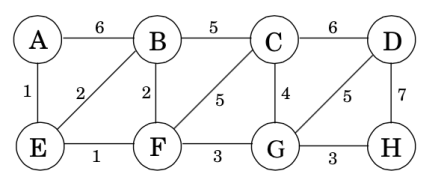
\includegraphics[width=3in]{DPV51.PNG}
\end{center}

\begin{enumerate}

\item What is the cost of it's minimum spanning tree? \\ The total cost of the minimum spanning tree is 14, it consists of the following edges :
$$ [(A,E,1), (E,B,2), (E,F,1), (F,G,3), (G,C,4), (G,H,3)] $$

\item How many minimum spanning trees does it have? \\ By Caley's theorem, there are $n^{n-2}$ spanning trees, given that $n=8$, the number of spanning trees is $8^6=262144$.

\item Suppose Kruskals algortithm is run on this graph. In what order are the edges added to the MST? For each edge in this sequence give a cut that justifies its addition. \\

Below is a table that answers the question above. It shows the steps of the algorithm going down the table, with the groups
of vertices being shown in the other columns. Notice they all start out as singletons before being formed into a single tree.
This example is odd in that no other components of size greater than one were created, all iterations consisted of adding a singleton to the current tree, which does not have to happen with Kruskal's algorithm. \\
\begin{tabular}{|c|c|c|c|c|c|c|c|c|} \hline
iteration & A & B & C & D & E & F & G & H \\ \hline
        1 & AE & B & C & D &  & F & G & H \\ \hline
        2 & AEF & B & C & D &  &  & G & H \\ \hline
        3 & AEFB &  & C & D &  &  & G & H \\ \hline
        4 & AEFBG &  & C & D &  &  &  & H \\ \hline
        5 & AEFBGH &  & C & D &  &  &  &  \\ \hline
        6 & AEFBGHC &  &  & D &  &  &  &  \\ \hline
        7 & AEFBGHCD &  &  &  &  &  &  &  \\ \hline 
\end{tabular}

\end{enumerate}

\end{homeworkProblem}





%----------------------------------------------------------------------------------------
%   PROBLEM 3
%----------------------------------------------------------------------------------------
\begin{homeworkProblem}
Often there are multiple shortest paths between two nodes of a graph. How do you need to
modify Dijkstra’s algorithm so that it finds the number of shortest paths

\end{homeworkProblem}





%----------------------------------------------------------------------------------------
%   PROBLEM 4
%----------------------------------------------------------------------------------------
\begin{homeworkProblem}

Recall that the correctness proof of Dijkstra’s algorithm assumes that the weights of the edges
are non-negative. Give a small example digraph with some negative edges where Dijkstra’s
algorithm does not find the shortest path.

\end{homeworkProblem}






%----------------------------------------------------------------------------------------
%   PROBLEM 5
%----------------------------------------------------------------------------------------
\begin{homeworkProblem}

KT, problem 17, p 197.)\\
Consider the following variation on the Interval Scheduling Problem.You have a processor that can operate 24 hours a day, every day. People submit requests to run \textit{daily jobs} on the processor. Each such job comes with a \textit{start time} and an \textit{end time}; if the job is accepted to run on the processor, it must run continuously, every day, for the period between its start and end times. (Note that certain jobs can begin before midnight and end after midnight; this makes for a type of situation different from what we saw in the Interval Scheduling Problem.)\\

Given a list of $n$ such jobs, your goal is to accept as many jobs as possible (regardless of their length), subject to the constraint that the processor can run at most one job at any given point in time. Provide an algorithm to do this with a running time that is polynomial in $n$. You may assume for simplicity that no two jobs have the same start or end times.\\

\textbf{Example.} Consider the following four jobs, specified by (\textit{start-time, end- time}) pairs.\\
\begin{displaymath}
\text{(6 PM, 6 AM), (9 PM, 4 AM), (3 AM, 2 PM), (1 PM, 7 PM)}
\end{displaymath}

The optimal solution would be to pick the two jobs (9 P.M., 4 A.M.) and (1 P.M., 7 P.M.), which can be scheduled without overlapping.

\end{homeworkProblem}






%----------------------------------------------------------------------------------------
%   PROBLEM 6
%----------------------------------------------------------------------------------------
\begin{homeworkProblem}

KT, Problem 2, p. 189
\end{homeworkProblem}



%----------------------------------------------------------------------------------------

\end{document}